\documentclass{fancyslides} 
\usepackage[utf8]{inputenc}
\usepackage{times}


%%% Beamer settings (do not change)
\usetheme{default} 
\setbeamertemplate{navigation symbols}{} %no navigation symbols
\setbeamercolor{structure}{fg=\yourowntexcol} 
\setbeamercolor{normal text}{fg=\yourowntexcol} 



%%%%%%%%%%%%%%%%%%%%%%%%%
%%% CUSTOMISATIONS %%%%%%
%%%%%%%%%%%%%%%%%%%%%%%%%

%%%% SLIDE ELEMENTS
\newcommand{\structureopacity}{0.75} %opacity for the structure elements (boxes and dots)
\newcommand{\strcolor}{blue} %elements colour (predefined blue; orange; green)

%%%% TEXT COLOUR
\newcommand{\yourowntexcol}{white}



%%%%%%%%%%%%%%%%%%%%%%%%%
%%% TITLE SLIDE DATA %%%%
%%%%%%%%%%%%%%%%%%%%%%%%%
\newcommand{\titlephrase}{MAKE YOUR POINT CLEAR WITH FANCYSLIDES}
\newcommand{\name}{Your Name}
\newcommand{\affil}{Company}
\newcommand{\email}{your.email@domain.com}





\begin{document}







\startingslide %this generates titlepage from the data above




\fbckg{1}
\begin{frame}
\pointedsl{your point}
\end{frame}


\fbckg{2}
\begin{frame}
\framedsl{explained clearly}
\end{frame}


\fbckg{2}
\begin{frame}
\itemized{
\item BEAMER EASE OF USE
\item MODERN LOOK \& FEEL
}
\end{frame}






\fbckg{2}
\begin{frame}
\framedsl{\pitem{pointed slogan} \pitem{framed slogan} \fitem{beamer features}}
\end{frame}







\fbckg{1}
\begin{frame}
  \thankyou   %%%% ending slide with thank you notice
\end{frame}





\fbckg{blank}
\begin{frame}
\sources{
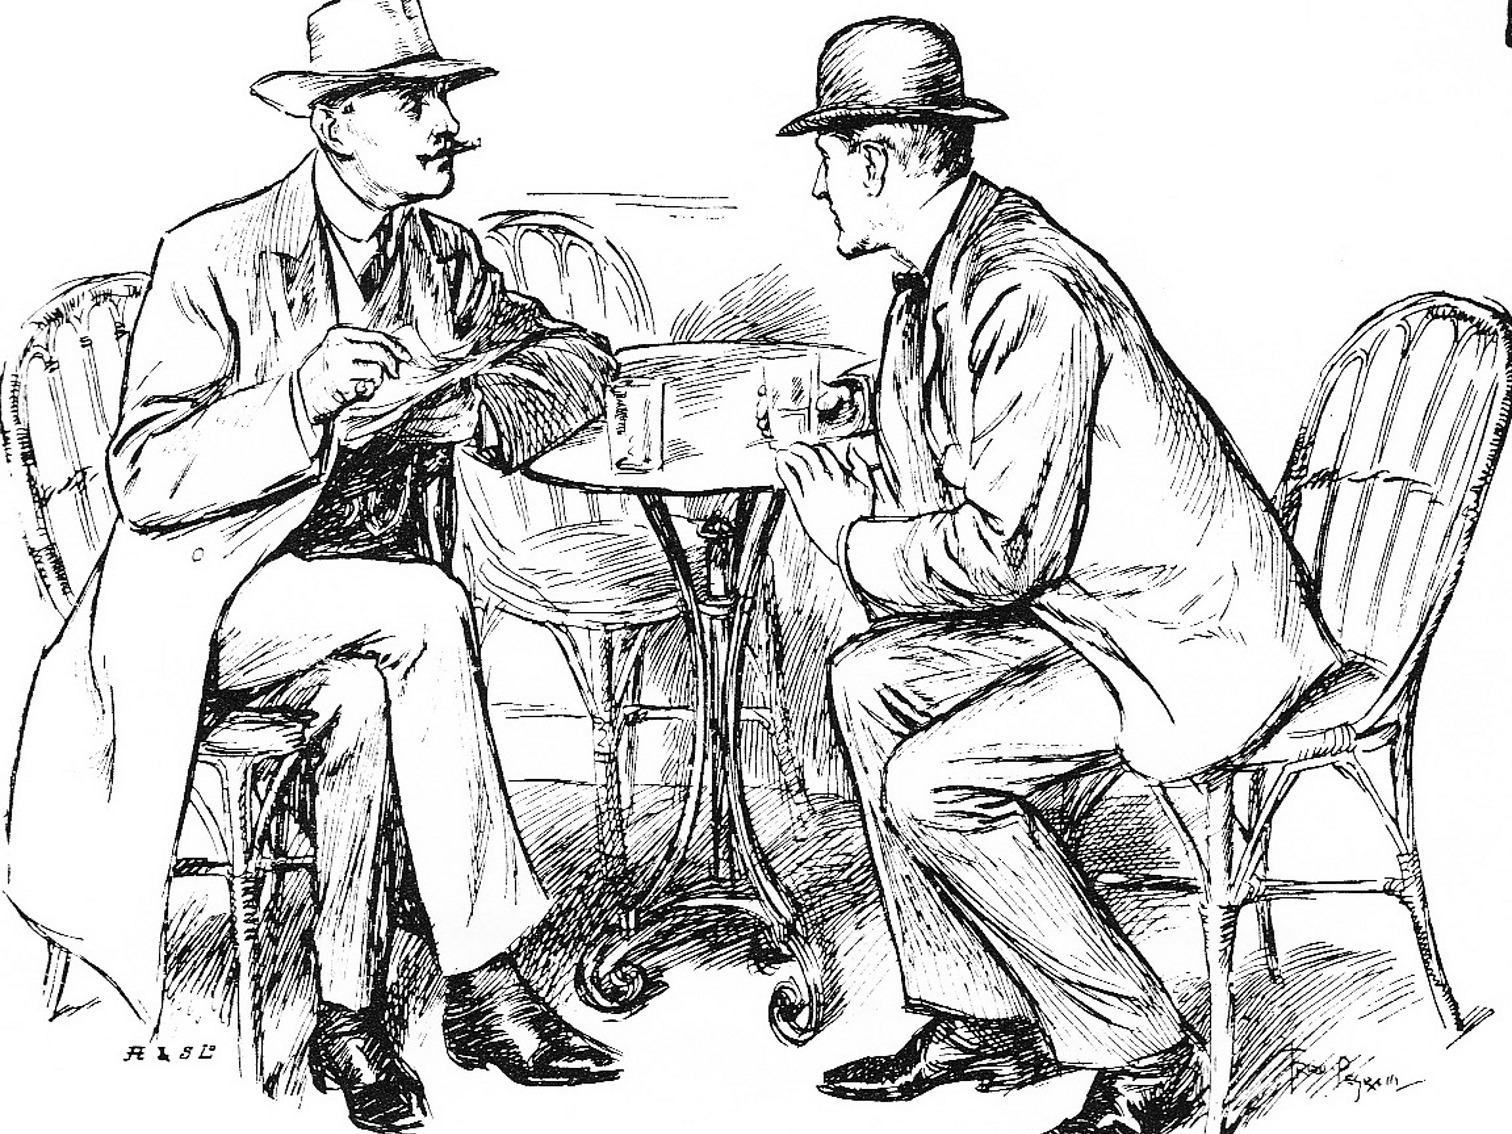
\includegraphics[scale=0.048]{1} \ flickr/lovelornpoets\\
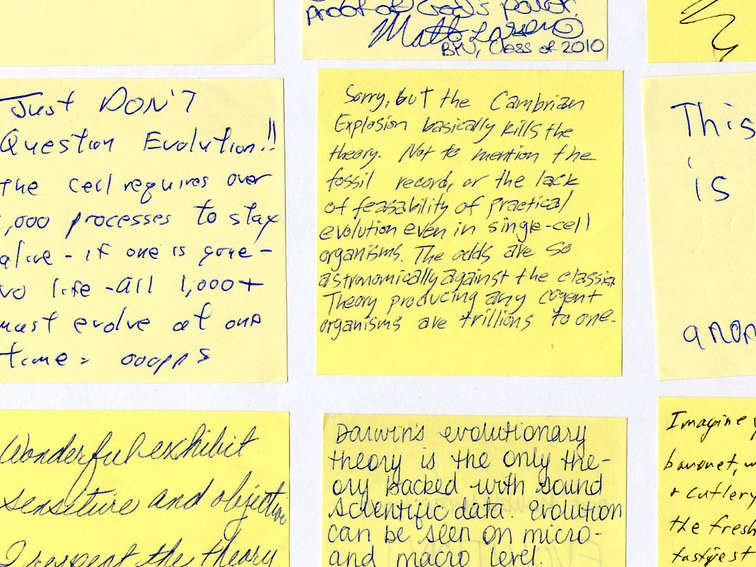
\includegraphics[scale=0.2]{2} \ flickr/apsmuseum
}
\end{frame}


\end{document}